\chapter{Spatial Profiling}
\label{ch:spatial-profile}
\section{Purpose}
\label{sec:spatial-profile-purpose}

A major concern with the practical application of TR to WPT is the ability of WPT to safely and consistently converge on its target.  An ideal TR WPT system will focus large amounts of energy on a very small space.  However, the question remains: how small of a space is it focused in?

The answer to this question will have major repercussions on the ability of TR to be used in a WPT context.  If the area of reconstruction is large, additional energy may be directed to the area around the target.  The increased energy density in this region will make losses due to absorption much higher than in other parts of the chamber.  More importantly however, this absorbed energy may damage circuitry or biological matter near the TR receiver.

Clearly, the spatial profile of a reconstruction should be as small as possible.  For TR WPT to be used on small electronic devices, the profile should be small enough not to damage circuits or biological matter within a centimeter or so of the device.  An experiment was done to characterize this behavior, as it exists in our setup.

\section{Methodology}
\label{sec:spatial-profile-meth}

Characterization of the spatial profile was done in the same aluminum cavity used in the linear and nonlinear time reversal tests, listed above.

The basic time reversal process in this environment proceeds as follows: First, a 50 ns Gaussian pulse (with a carrier frequency of 5 GHz) is injected into the cavity through the transmitting antenna. That sona is measured at the receiving antenna (Fig. 1b). The sona is then time reversed and injected into the transmitting antenna. The result is a reconstruction of the initial pulse back at the receiving antenna (Fig. 1c). This process makes use of another robust symmetry, namely the spatial reciprocity of the wave equation.
Two monopole antennas inject and extract electromagnetic signals from different points in the enclosure. A transmitting antenna is attached to the cavity wall opposite the receiving antenna. The receiving antenna is attached to a panel that can move vertically with a total range of 70 millimeters. Motion of the receiving antenna is achieved using an externally-mounted PI MikroMove \texttt{M-415.DG} translation stage and the enclosure remains sealed during the translation. Interrogation pulses and time-reversed sona signals are created and broadcast using a Tektronix \texttt{AWG7052} arbitrary waveform generator feeding an Agilent \texttt{E8267D} Vector PSG microwave source. A digital storage oscilloscope (DSO, Agilent \texttt{DSO91304A}) is used to record waveforms of interest. MATLAB is used for signal processing and instrument control and coordination.

\section{Results}
\label{sec:spatial-profile-results}

\begin{figure}[t!]
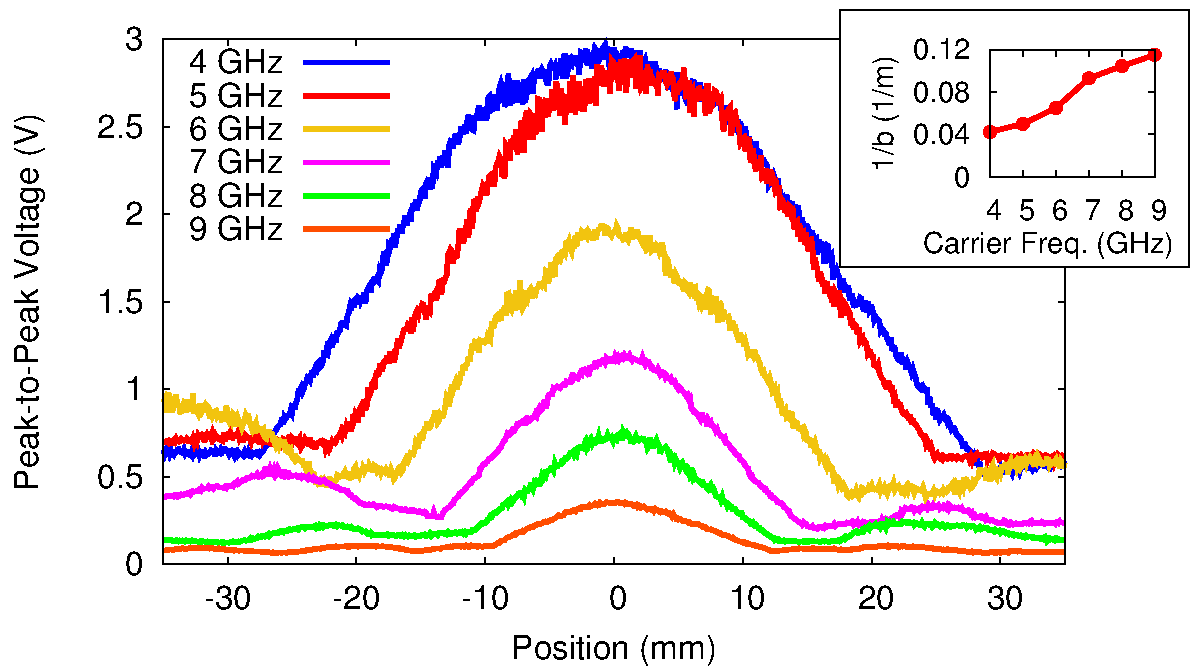
\includegraphics[width=\columnwidth]{spatial/freq_profile.pdf}
\caption{Spatial profile of peak-to-peak voltage amplitudes of reconstructions
investigated at carrier frequencies ranging from 4 to 9 GHz in 1 GHz
steps.  The inset shows the inverse of the fit $b$ values versus carrier frequency, showing the expected linear relationship.}
\label{fig:spatial-freq-profile}
\end{figure}

The first experiment measures the spatial profile of a reconstruction, with the goal of characterizing reconstruction size as a function of carrier signal wavelength. A reconstruction is focused on the receiving antenna, in the middle of its movement range. Without changing the time reversed sona being broadcast, the receiving antenna is systematically translated through its entire range of movement. Samples are taken every 0.2 mm across the entire 70~mm range, and the maximum peak-to-peak voltage of the corresponding reconstruction is recorded at each step. We repeated this experiment for carrier frequencies in the range 4-9 GHz and display these results in Figure~\ref{fig:spatial-freq-profile}.

\section{Discussion}
\label{sec:spatial-profile-discussion}

\begin{figure}[t!]
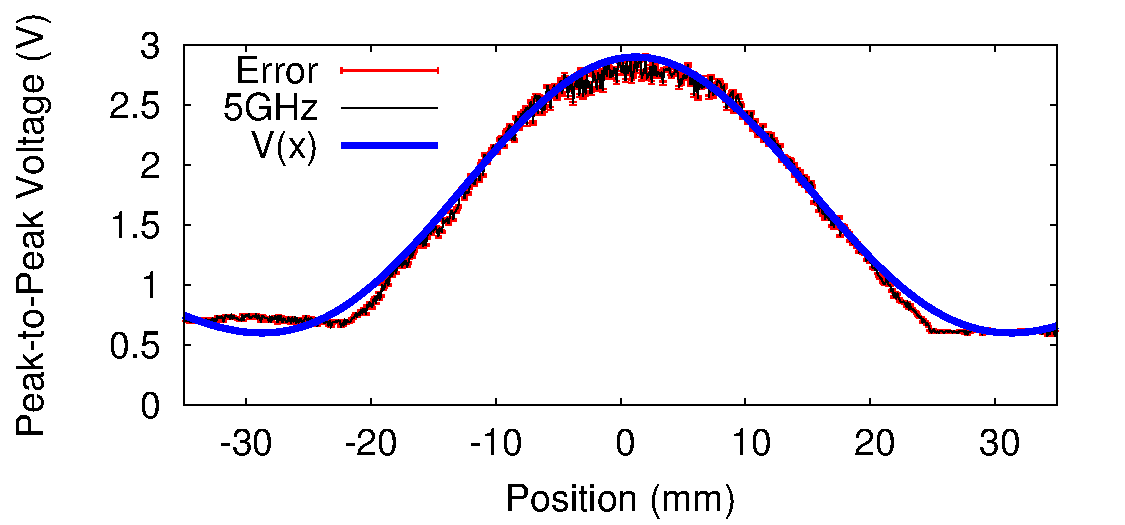
\includegraphics[width=\columnwidth]{spatial/fit.pdf}
\caption{Measured peak-to-peak voltage amplitude of reconstructions received in the
vicinity of a time-reversed wave collapse location with a 5 GHz carrier
frequency, and fit to the \texttt{sinc(x)} function.}
\label{fig:spatial-error-fit}
\end{figure}

The reconstruction peak-to-peak voltage profile is expected to take the form of a $sinc(x)$ function about the antenna~\ref{cite:lerosey-focusing}. Thus, the following equation is proposed to predict $V(x)$, the maximum peak-to-peak voltage from a given reconstruction, as a function of $x$, the distance between the reconstruction focal point and the receiver:

\begin{equation}
\label{eq:vx}
V(x) = a\cdot sinc\left(\frac{x+c}{b}\right) + d
\end{equation}

where $a$ is the maximum peak-to-peak reconstruction amplitude, $b$ is the wavelength of the signal divided by 2, $c$ is the location of the antenna along the x-axis, and $d$ is the noise level
offset voltage. Since $b$ is proportional to the wavelength (and inversely proportional
to frequency), as the carrier frequency is increased,  $\frac{1}{b}$ also increases, causing the ``bubble'' of the sinc function in Fig~\ref{fig:spatial-freq-profile} to get smaller. This relationship is shown explicitly in the inset of Figure~\ref{fig:spatial-freq-profile}. Figure~\ref{fig:spatial-error-fit} shows Equation~\ref{eq:vx} fit to the 5 GHz curve from Figure~\ref{fig:spatial-freq-profile}, including error bars. The fit is good, but has a reduced $\chi^2$ of 234 due in part to the rather large background noise level. The error bars are primarily systematic, introduced by the oscilloscope internal voltage multiplier used in scaling.
